\section{OctoPrint API}

V implementační části práce se zabývám vytvořením mobilní aplikace pro OctoPrint.
Pro pro olvádání tiskárny využiji REST API, které OctoPrint v základu nabízí.
V dalších sekcích se budu podrobně zabývat analýzou jednotlivých funkcionalit implementovaných v mém řešení.

Z důvodu bezpečnosti musí být každý požadavek na tiskárnu autorizovaný.
To OctoPrint zajišťuje pomocí ověřovacích \textit{tokenů}.
Token je náhodně vygenerovaná posloupnost znaků jednoznačně spjatá s účtem uživatele.
Pokud v požadavku je uveden platný token, předpokládá se, že požadavek vytvořil uživatel jehož účet je s token svázaný.

V analýze jsem vycházel z oficiální dokumentace aplikace OctoPrint \cite{octoprint-docs}.
Ukázka popisu funkcionality z dokumentace je vidět v obrázku \ref{fig:octoprint-docs}.

\begin{figure}\centering
	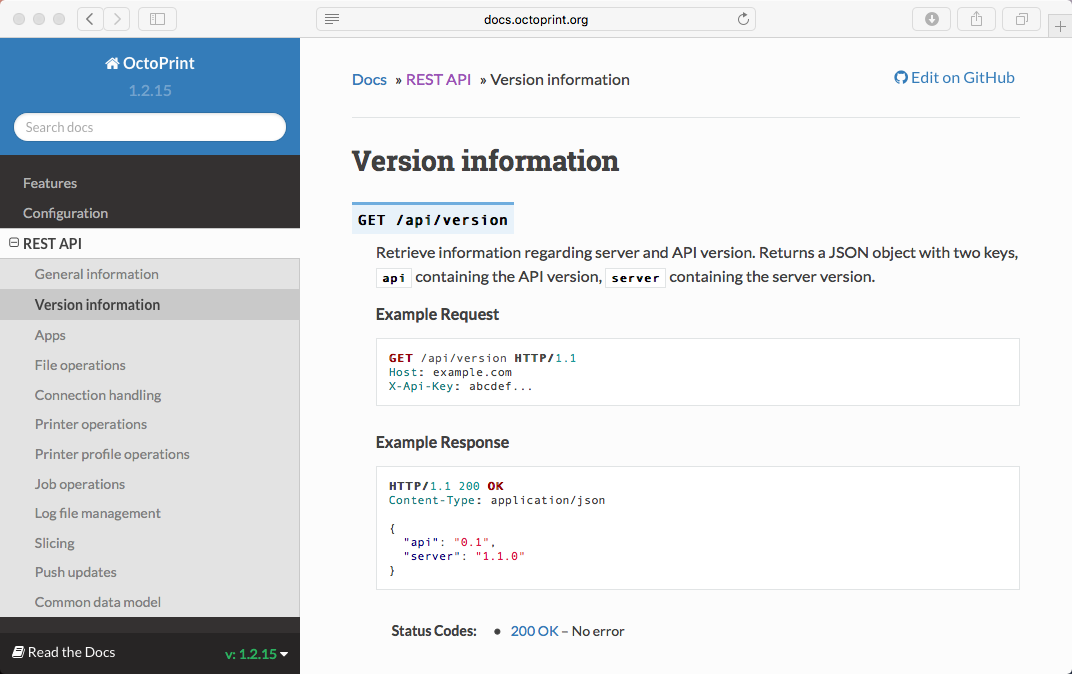
\includegraphics[width=\textwidth]{assets/analysis-octoprintapi-web.png}
	\caption{Oficiální dokumentace OctoPrint}\label{fig:octoprint-docs}
\end{figure}

\subsection{Verze API a ověřování}

První analyzovanou funkcionalitou je verze API.
Tento endpoint je dostupný na \inlinestr{api/version}.
V případě platného přístupového tokenu vrátí textovou reprezentaci verze API, v opačném případě odpovídající stavový kód.

Ve své implementaci jsem se rozhodl uživatele nezatěžovat využívanými verzemi.
Jedná se ale o jediný endpoint, který nemá žádné vedlejší efekty.
Zároveň neexistuje žádný endpoint umožňující samostatně ověřit platnost tokenu.

Vzhledem k výše uvedenému je tato funkcionalita vhodná pro simulaci přihlašování k tiskárně.

\subsection{Správa souborového systému}

Jednou ze skupin funkcionalit REST API je správa souborového systému.
Pomocí API lze nejen obsah systému číst, ale také s ním manipulovat.
Jednotlivé endpointy jsou zanalyzovány níže.

\subsubsection*{Seznam souborů}

OctoPrint umožňuje vypsat seznam uložených souborů.
Tento endpoint je dostupný na \inlinestr{api/files}.

V současnou chvíli mohou na soborový systém být uloženy pouze tisknutelné soubory (s příponou .gcode) nebo modelové soubory (s příponou .stl).

Uloženy mohou být přímo na zařízení kde je OctoPrint nainstalovaný (označované jako lokální) nebo na paměťovou kartu.
Výše zmíněná funkce stáhne seznam všech souborů bez ohledu na jejich lokace.
Příznak lokace je v odpovědi uveden u každého souboru zvlášť.

Lze ale stáhnout soubory z obou lokalit samostatně.
Pro stažení seznamu lokálních souborů existuje koncový bod \inlinestr{api/files/local}.
Seznam ouborů uložených na paměťové kartě je možné stáhnout z \inlinestr{api/files/sdcard}.

O souborech jsou dostupná jejich metadata (název, velikost, datum změny).
GCode může navíc obsahovat analýzu tisku (předpokládaná doba tisku, spotřeba filamentu a statistiky tisknutí).

Struktura odpovědí je pro všechny tři požadavky stejná, liší se pouze obsah seznamu v závislosti na vybrané lokalitě.

\subsubsection*{Nahrávání souborů}

Pomocí API je možné nejen číst informace o existujících souborech, ale také nahrávat nové.
Pro nahrávání slouží endpointy \inlinestr{api/files/local} a \inlinestr{api/files/sdcard}.
Podle zvoleného koncového bodu se soubor uloží buď přímo na zařízení nebo na paměťovou kartu.

Soubor se odesílá v těle požadavku kde je zároveň uveden jeho název.
V případě vzniku konfliktu názvů bude stávající soubor nahrazen novým.

Systém iOS neobsahuje sdílený souborový systém, soubory lze nahrávat buď pouze z aplikace nebo lze využít cloudových služeb \cite{apple-file-system-basics}.

\subsubsection*{Informace o konkrétním souboru}

Aby bylo možné aktualizovat informace o jednotlivých souborech, umožňuje OctoPrint využít koncový bod \inlinestr{api/files/[location]/[filename]}.
Takový požadavek zajistí stažení aktuálních informací o souboru v lokaci \textit{[location]} s názvem \textit{[filename]}.

Strukturou se odpověď nelyší od položky souboru v seznamu souborů.
Požadavek lze ale využít v momentě, kdy se z klientské aplikace se souborem v tiskárně manipuluje pro udržení konzistence.

\subsubsection*{Manipulace se soubory -- Tisk}

OctoPrint umožňuje pro manipulaci se soubory více konfigurací.
Pro využití v mobilní aplikaci se ale hodí pouze konfigurace pro tisk.
Ta je dostupná na endpointu \inlinestr{api/files/[location]/[filename]}.

V těle požadavku je nutné uvést typ příkazu a explicitně vyžádat tisknutí.
Více o konfiguracích se lze dočíst v dokumentaci \cite{octoprint-api-filecommand}.

\subsubsection*{Smazání souboru}

Další funkcionalitou je odstranění souboru.
Tento endpoint je dostupný na \inlinestr{api/files/[location]/[filename]}.
Požadavek je nutné odeslat metodou \textit{DELETE}.

\subsection{Připojení tiskárny}

Protože OctoPrint běží na samostatném zařízení a hardware tiskárny jen ovládá, je nutné ho k tiskárně explicitně připojit.
Připojení probíhá pomocí výběru dostupného portu.
Seznam dostupných portů poskytuje sám OctoPrint.

\subsubsection*{Nastavení připojení}

Pomocí koncového bodu \inlinestr{api/connection} lze zjistit akuální nastavení připojení k tiskárně.
Přestože tato informace není ztěžejní pro mobilní aplikaci, odpověď serveru na tento požadavek obsahuje seznam portů.

Seznam portů lze využít pro výzvu uživatele v momentě o připojení tiskárny.
To může nastat v momentě kdy uživatel chce s tiskárnou pracovat v době kdy žádná tiskárna připojena není.

\subsubsection*{Příkaz připojení tiskárny}

Podobně jako v sekci o manipulaci souborů, i tento endpoint nabízí mnoho konfigurací.
Pro mobilní aplikaci ale nedávají z důvodu komplikovaného nastavení velký smysl.

Zajímavou konfigurací je ale možnost připojit tiskárnu.
Tento koncový bod se nalézá na \inlinestr{api/connection} a jako metodu je nutné využít \textit{POST}.

V těle požadavku musí být explicitně zadaný příkaz \textit{connect} a také port pro připojení.
Hodnota portu musí být jedna z uvedených v seznamu portů.
Seznam portů je možné získat z nastavení připojení.

\subsection{Ovládání tiskárny}

Ovládání tiskárny je docíleno pomocí příkazů jednotlivým částem tiskárny.
Ve verzi API \vapi jsou rozpoznávány následující příkazy následujícím částem:

\begin{description}
	\item[Tisková hlava] Umožňuje pohybovat tiskovou hlavou tiskárny po všech třech osách.
	\item[Tryska] Umožňuje nastavení teplot trysky.
	\item[Podložka] Umožňuje nastavení teplot podložky.
	\item[Paměťová karta] Dovoluje manipulovat s přijením paměťové karty v momentě, kdy je dostupná.
\end{description}

\subsubsection*{Aktuální stav tiskárny}

Prvním analyzovaným koncovým bodem této skupiny je aktuální stav tiskárny.
Ten je dostupný na \inlinestr{api/printer}.
Odpověď obsahuje informace o teplotách podložky a tryskové hlavy.
Dále lze v odpovědi nalézt informace o celkové připravenosti tiskárny.

Tento endpoint je vhodný pro obrazovku s přehledem stavu tiskárny.

\subsubsection*{Ovládání trysky}

Ovládání trysky je nastavitelný endpoint přístupný na \inlinestr{api/printer/tool}.
Každý požadavek na tento koncový bod musí být odeslaný metodou \textit{POST}.

Z důvodu zjednodušení uživatelského rozhraní jsem se rozhodl analyzovat nastavení pro tavení filamentu.
Toto nastavení vyžaduje explicitně zadat příkaz pro tavení a množství filamentu, které má být nataveno.

Tato funkce je ideální pro zkombinování s ovládáním tiskové hlavy.

\subsubsection*{Aktuální stav trysky}

Pro kontrolu správného průběhu tisku je důležité sledovat teplotu trysky.
OctoPrint nabízí z tohoto důvodu endpoint \inlinestr{api/printer/tool}.
V odpovědi se nachází informace o akuální teplotě.

\subsubsection*{Ovládání podložky}

Podobně jako u trysky je možné konfigurovat teplotu i u podložku.
Koncový bod se nachází na \inlinestr{api/printer/bed}, požadavek je nutné vytvořit metodou \textit{POST}.

\subsubsection*{Aktuální stav podložky}

OctoPrint nabízí také informace o aktuální teplotě podložky.
Endpoint je dostupný na \inlinestr{api/printer/bed}.

Tyto informace je možné zobrazit na přehledu stavu tiskárny.

\subsubsection*{Ovládání paměťové karty}

Aby bylo možné manuálně spravovat stav paměťové karty, nabízí OctoPrint koncový bod \inlinestr{api/printer/sd}
Pomocí této funkce lze paměťovou kartu připojit, odpojit nebo vynutit načtení dat.

Jednotlivé konfigurace je nutné v požadavku explicitně uvést.
Každý požadavek musí být metodou \textit{POST}.

\subsubsection*{Aktuální stav paměťové karty}

Pro možnost informovat uživatele o akutálním stavu paměťové karty je dostpuný koncový bod \inlinestr{api/printer/sd}.
Odpověď vrací booleovskou hodnotu indikující je-li karta připravena či ne.

\subsection{Tiskové profily}

OctoPrint umožňuje spravovat tiskové profily, pomocí nichž lze definovat fyzické vlastnosti tiskárny.
Mezi tyto vlastnosti patří informace o podložce, maximální rychlost tiskové hlavy či obsah tiskového profilu.

Tiskové profily nejsou v mé implementaci stěžejní funkcí, rozhodl jsem se proto i analýzu nepokrývat podrobně.
API poskytuje standardní \textit{CRUD} rozhraní pro správu profilů.
Je tedy možné profily vytvářet, číst, aktualizovat a mazat.
Rozhraní jsou dostupná na \inlinestr{api/printerprofiles}.
Jednotlivým požadavkům pak odpovídají HTTP metody podle CRUD standardu.

Více informací je možné získat z oficiální dokumentace \cite{octoprint-docs-printer-profiles}, i ta je ale na toto téma velmi skromná.

\subsection{Aktuální tisk}

Jednou z nejzajímavějších funkcí OctoPrint pro mobilní aplikaci je aktuální tisk.
Uživatel může jednoduše zkontrolovat, že tisk probíhá v pořádku, případně jak dlouho bude tisk ještě trvat.

\subsubsection*{Informace o aktuálním tisku}

Informace o aktuálním tisku jsou dostupné pomocí koncového bodu \inlinestr{api/job}.
Odpověď od serveru obsahuje metadata tisknutého souboru, odhad zbývajícího času a spotřebu materiálu.
Dále lze získat také informace o průběhu, tedy kolik procent je hotovo a jak dlouho se soubor tiskne.

\subsubsection*{Ovládání aktuálního tisku}

Ovládání tisku obsahuje mnoho konfigurací.
Pro mobilní aplikaci jsem zvolil možnost konfigurace pro zrušení tisku.
Pro zrušení aktuálního tisku je dostupný endpoint \inlinestr{api/job} s metodou \textit{POST}.
Do těla požadavku je nutné explicitně vložit příkaz pro zrušení tisku.
Více informací o konfiguracích je dostupné v dokumentaci \cite{octoprint-docs-job}.

\subsubsection*{Vlastní příkaz tiskárně}

Protože OctoPrint nepokrývá veškeré funkce tiskárny samostatnými konocovými body, je dostupný endpoint pro odeslání vlsatního příkazu tiskárně v jazyce GCode.

Tento koncový bod je dostupný na \inlinestr{api/printer/command}.
Vlastní příkaz se vkládá do těla požadavku.
Požadavek je nutné vytvořit metodou \textit{POST}.

Tato funkcionalita je vhodná pro vytvoření obrazovky s vlastní terminálovým emulátorem.

\subsection{Správa log souborů}

Užitečnou funkcí OctoPrint je zobrazování logů.
OctoPrint seskupuje logy ze svého používání spolu s logy svých služeb (např. ze \textit{slicovacích nástrojů}).

\subsubsection*{Seznam logů}

Jednou z poskytovaných funkcí je seznam logů.
V seznamu je obsaženy metadata souboru a jeho umístění na souborovém systému.
Seznam je dostupný z přístupového bodu \inlinestr{api/logs}.

OctoPrint nenabízí samostatný endpoint pro detail logu, pro zobrazení obsahu je tedy nutné soubor stáhnout a teprve následně zobrazit.

\subsubsection*{Smazání logového souboru}

Z důvodu zvětšujícího se počtu souborů nabízí OctoPrint možnost manuálně mazat logy.
Mazání je možné pomocí endpointu \inlinestr{api/logs/[filename]} metodou \textit{DELETE}.

\subsection{Správa slicing profilů}

Obdobně jako u tiskových profilů nejsou slicing profily stěžejní funkcí.
Vzhledem k jejich složité konfigurace by jejich tvoření z mobilní aplikace mohlo působit špatný uživatelský zážitek.
Z tohoto důvodu jsem neprováděl podrobnou analýzu této funkcionality.

OctoPrint nabízí koncový \inlinestr{api/slicing}, na kterém jsou dostupné CRUD operace.
Manipulace je tedy možná pomocí dalších funkcí z nichž každá operuje s odpovídající HTTP metodou.

Podrobné informace k jednotlivým funkcím jsou dostupné v oficiální dokumentaci \cite{octoprint-docs-slicing}.
